
\chapter{\label{cha:Analytical-Solns}Analytical Solutions}


\section{\label{sec:TractionProblems}Traction Problems}

Computation of analytical solutions for elastostatic problems over
regular domains is a relatively straightforward procedure. These problems
are typically formulated in terms of a combination of displacement
and traction boundary conditions, and such problems provide a good
test of the code accuracy, as well as specifically testing the implementation
of traction boundary conditions. We present here two simple problems
for this purpose.


\subsection{Solutions Using Polynomial Stress Functions}

Our derivation follows the procedures outlined in Timoshenko and Goodier
\cite{Timoshenko:Goodier:1987}, and we restrict ourselves to two-dimensional
problems. Any problem in elastostatics must satisfy the equilibrium
equations
\begin{gather}
\frac{\partial\sigma_{xx}}{\partial x}+\frac{\partial\sigma_{xy}}{\partial y}+X=0\label{eq:traction:1}\\
\frac{\partial\sigma_{yy}}{\partial y}+\frac{\partial\sigma_{xy}}{\partial x}+Y=0,\nonumber 
\end{gather}
where \textit{X} and \textit{Y} are the body force components in the
\textit{x} and \textit{y} directions, respectively, and the stress
components are given by $\sigma$. In the problems considered here,
we neglect body forces, so \textit{X} and \textit{Y} disappear from
the equilibrium equations. The solution must also satisfy the boundary
conditions, given as surface tractions over the surface of the body.
Finally, the solution must satisfy the conditions of compatibility,
which may be expressed as:
\begin{equation}
\left(\frac{\partial^{2}}{\partial x^{2}}+\frac{\partial^{2}}{\partial y^{2}}\right)\left(\sigma_{xx}+\sigma_{yy}\right)=0.\label{eq:traction:2}
\end{equation}
To compute the displacement field, it is also necessary to specify
displacement boundary conditions.

Equations \vref{eq:traction:1} may be satisfied by taking any function $\phi$
of \textit{x} and \textit{y}, and letting the stress components be
given by the following expressions:
\begin{equation}
\sigma_{xx}=\frac{\partial^{2}\phi}{\partial y^{2}},\;\sigma_{yy}=\frac{\partial^{2}\phi}{\partial x^{2}},\;\sigma_{xy}=-\frac{\partial^{2}\phi}{\partial x\partial y}.\label{eq:traction:3}
\end{equation}
The solution must also satisfy the compatibility equations. Substituting
Equations \vref{eq:traction:3} into Equation \vref{eq:traction:2}, we find that the
stress function $\phi$ must satisfy
\begin{equation}
\frac{\partial^{4}\phi}{\partial x^{4}}+2\frac{\partial^{4}\phi}{\partial x^{2}\partial y^{2}}+\frac{\partial^{4}\phi}{\partial y^{4}}=0.\label{eq:traction:4}
\end{equation}
A relatively easy way to solve a number of problems is to select expressions
for $\phi$ consisting of polynomial functions of \textit{x} and \textit{y}
of second degree or higher. Any polynomial of second or third degree
will satisfy Equation \vref{eq:traction:4}. For polynomials of higher degree,
they must be substituted into Equation \vref{eq:traction:4} to determine what
restrictions must be placed on the solution.


\subsection{\label{sub:Analytical-Constant-Traction}Constant Traction Applied
to a Rectangular Region}

For this problem, a constant normal traction, $\overrightarrow{N}$,
is applied along the positive \textit{x}-edge of the rectangular region
($x=x_{0}$), and roller boundary conditions are applied along the
left and bottom boundaries (\vref{fig:Const-tractions}). Since the
tractions are constant, we assume a second degree polynomial for the
stress function:
\begin{equation}
\phi_{2}=\frac{a_{2}}{2}x^{2}+b_{2}xy+\frac{c_{2}}{2}y^{2}.\label{eq:traction:5}
\end{equation}
This yields the following expressions for the stresses:
\begin{equation}
\sigma_{xx}=\frac{\partial^{2}\phi_{2}}{\partial y^{2}}=c_{2}=N,\;\sigma_{yy}=a_{2}=0,\;\sigma_{xy}=-b_{2}=0.\label{eq:traction:6}
\end{equation}
From Hooke's law, we have:
\begin{equation}
\epsilon_{xx}=\frac{\partial u}{\partial x}=\frac{\left(1-\nu^{2}\right)N}{E},\;\epsilon_{yy}=\frac{\partial v}{\partial y}=\frac{-\nu\left(1+\nu\right)N}{E},\;\epsilon_{xy}=\frac{1}{2}\left(\frac{\partial v}{\partial x}+\frac{\partial u}{\partial y}\right)=0.\label{eq:traction:7}
\end{equation}
The strain components are thus easily obtained from the stress components.

To obtain the displacements, we must integrate Equation \vref{eq:traction:7}
and make use of the displacement boundary conditions. Integrating
the first two of these, we obtain
\begin{equation}
u=\frac{\left(1-\nu^{2}\right)Nx}{E}+f\left(y\right),\; v=\frac{-\nu\left(1+\nu\right)Ny}{E}+f\left(x\right).\label{eq:traction:8}
\end{equation}
Substituting these into the third expression, we obtain
\begin{equation}
\frac{\partial f\left(x\right)}{\partial x}=-\frac{\partial f\left(y\right)}{\partial y},\label{eq:traction:9}
\end{equation}
which means that both $f\left(x\right)$ and $f\left(y\right)$ must
be constant. We solve for these constants using the displacement boundary
conditions along $x=x_{0}$ and $y=y_{0}$. Doing this, we obtain
the following expressions for the displacement components:
\begin{equation}
u=\frac{\left(1-\nu^{2}\right)N}{E}\left(x-x_{0}\right),\; v=\frac{\nu\left(1+\nu\right)N}{E}\left(y_{0}-y\right).\label{eq:traction:10}
\end{equation}


\noindent \begin{center}
\begin{figure}[H]


\caption{\label{fig:Const-tractions}Problem with constant traction boundary
conditions applied along right edge.}


\noindent \centering{}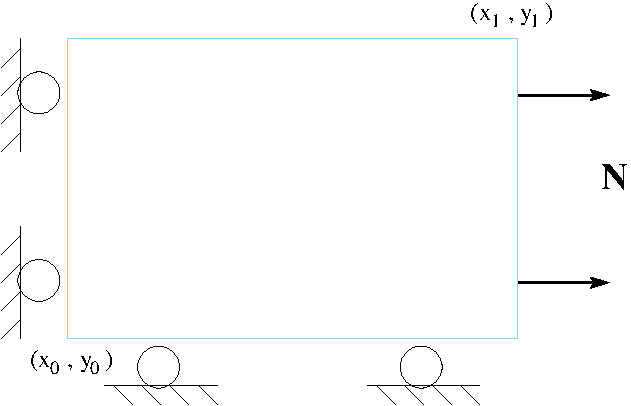
\includegraphics{analyticalsolns/figs/consttract}
\end{figure}

\par\end{center}
